\begin{figure}[t]
  \centering
  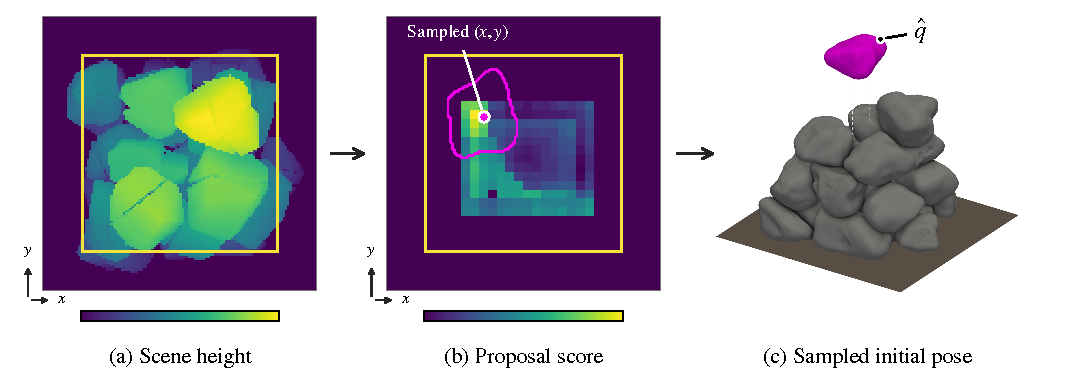
\includegraphics[width=\columnwidth]{figures/initial_pose_sampling.pdf}
  \caption{Initial pose sampling for a fixed object and orientation: (a) scene height, (b) proposal score and sampled planar location, and (c) initial pose $\hat q$ above the scene. Magenta links the sampled location and candidate object.}
  \label{fig:score_map}
\end{figure}

\section{Sequence Planning} \label{sec:sequence_planning}

\subsection{Initial Pose Sampling}
The sampler $\initpose$ allocates fresh proposals to remaining objects in proportion to their volumes and considers a finite set of orientation hypotheses for each object. It prioritizes connected growth on the lowest incomplete layer, seeding an empty scene near feasible target corners. For an object $i$, orientation $R$, and feasible planar location $\planar$, the geometric score is
\begin{equation*}
  \score(\planar\mid i,R)
  =w_\text{s}\score_\text{s}+w_\text{f}\score_\text{f}
   +w_\text{b}\score_\text{b}-w_\text{h}\score_\text{h},
\end{equation*}
with positive weights. The terms measure the fraction of bottom samples near predicted contact, unfilled layer area beneath the footprint, proximity to the feasible placement boundary, and normalized mean contact height, respectively. The floor and boundary preferences are inspired by Menezes et al.~\cite{menezes2021rocks}. Figure~\ref{fig:score_map} illustrates the resulting proposal score and sampled initial pose.

Within eligible pools, the standard sampler combines elite selection with draws without replacement weighted by $\exp(\score/\tau)$, $\tau>0$. Each selected hypothesis is initialized above overlapping scene geometry with a clearance, then refined by $\poseopt$ and filtered for feasibility. At the search root, population refinement additionally mixes fresh proposals with planar-position and yaw mutations of promising candidates, followed by renewed pose optimization.
% Standard sampler: volume-biased budgets, platform-specific orientation banks,
% active-layer/connectivity masks, elite fraction 0.25, temperature 0.3.
% Contact height used for scoring differs from the lifted optimization seed.
% Composite sampling has region-local masks/layers and currently greedy draws
% within each eligible region.

\subsection{Simulation Module}\label{sec:simulation}
The module $\simul$ evaluates every proposed transition using the same simulation procedure at all search depths.
It first settles the new object for a fixed duration while holding the existing objects static.
From the resulting poses, it resets velocities and simulates the entire structure's response to the added load.
Structural simulation requires a minimum duration and sustained low mass-normalized kinetic energy.
Excessive accumulated motion, invalid contacts, or failure to settle within the time limit rejects the placement.

For an accepted nominal simulation, the settled scene defines the successor $\state'=\transition(\state,\action)$.
Separate trials start from this scene by perturbing the new object's initial twist with independent samples $\xi_j\sim\mathcal{N}(0,\Sigma)$ in $\mathfrak{se}(3)\simeq\mathbb{R}^6$, where $\Sigma$ is the velocity covariance.
Each perturbation is applied once at the start of trial $j$.
To reduce computation, only the candidate and stones within two links in the nominal scene's contact graph of movable stones remain dynamic throughout each trial.
All other bodies retain fixed collision geometry.
These trials estimate local robustness without changing $\state'$.
The resulting successor, reward, and feasibility outcome are stored in the tree and used directly for subsequent search and action selection.
Simulation uses CUDA subADMM~\cite{ji2025gpu}.
% Quiet proxy: e_l = 2 K_l / m_l; motion integral = integral sqrt(e_l) dt.
% Disturbance magnitudes, quiet windows, timeouts, and mobility settings are
% experimental parameters, not a calibrated model of release uncertainty.

\subsection{Reward Design}
For the newly placed object $i=i_{k+1}$, let $q_i'$ be its pose in the settled successor $s'$ returned by $\simul$ (Sec.~\ref{sec:simulation}). We define the target-volume and object-volume ratios
\begin{equation*}
 \rho_\target=\frac{\vol\bigl(\object_i(q_i')\cap\target\bigr)}{\vol(\target)},
 \quad
 \rho_\object=\frac{\vol\bigl(\object_i(q_i')\cap\target\bigr)}{\vol(\object_i)}.
\end{equation*}
The former measures the new object's contribution to filling the target; the latter measures its containment. Intersection volumes are estimated on a voxel grid. With fixed normalization scales absorbed into positive weights, the standard excavator reward is
\begin{equation*}
\begin{split}
 r(\state,\action)={}&w_\target\rho_\target+w_\object[\rho_\object-\tfrac12]_+
 -w_E e(\action)\\
 &-w_H\bigl(\max_{\Omega}H_{\state'}-\langle H_{\state'}\rangle_{\Omega}\bigr)
 -w_D D,
\end{split}
\end{equation*}
where $[x]_+=\max(x,0)$, so the containment bonus is active above $50\%$. Coverage lost through motion of earlier objects is not subtracted. $H_{\state'}$ is surface height over the target footprint $\Omega$, with zero at empty cells; $\langle\cdot\rangle_\Omega$ is its spatial mean.

The equilibrium score uses residual forces $\mathbf f_l$ and torques $\boldsymbol\tau_l$ returned by pose optimization:
\begin{equation*}
 e(\action)=\min\!\left\{1,\max_l\left(
 \frac{\|\mathbf f_l\|}{m_lg}
 +\frac{\|\boldsymbol\tau_l\|}{m_lg\vol(\object_l)^{1/3}}\right)\right\}.
\end{equation*}
Here $l$ indexes objects in the resulting structure and $g$ is gravitational acceleration.
Let $q_l(t;\xi_j)$ denote object $l$'s pose under the Gaussian velocity disturbance $\xi_j$ (Sec.~\ref{sec:simulation}), starting from its nominal successor pose $q_l'$.
Disturbance sensitivity is
\begin{equation*}
 D=\min\!\left\{D_{\max},\max_{j,l,t}d_{\SE(3)}\bigl(q_l(t;\xi_j),q_l'\bigr)\right\},
\end{equation*}
where $d_{\SE(3)}$ sums Euclidean translation distance and angular distance weighted by $\lambda_\theta>0$.
The maximum spans sampled disturbances, objects $l$ in this local dynamic neighborhood, and simulation time; $D_{\max}$ caps the penalty. Physical rejection criteria apply independently of the reward.
% Fixed scales are absorbed into paper weights, preserving the implemented reward.
% With Vbar = mean initial object volume and L = Vbar^(1/3), excavator:
% (w_T,w_O,w_E,w_H,w_D) = (vol(T)/Vbar,2,2,2/L,2/D_ref).
% Vbar is fixed for the initial inventory, not recomputed at each placement.
% Containment-ratio clipping is a numerical safeguard for voxel estimates, omitted from
% the geometric definition above (user agreement). The weight equivalence
% applies to the geometric reward; runtime estimates retain their safeguards.
% Tabletop additionally enables inward-orientation reward. Composite reward
% excludes previously occupied successor voxels and uses masked footprint means.
% Those variants are not interchangeable with a parent-to-successor union delta.

\subsection{Monte Carlo Tree Search}
We integrate these modules in batched, receding-horizon MCTS (Fig.~\ref{fig:overview}), following the parallel evaluation approach of~\cite{huang2022pmbs}.

\noindent \textbf{Batched Selection.}
For an optimized action $a=(i,q)$, let $\rho_\object^{\mathrm{pre}}$ denote the object-volume ratio evaluated at $q$, before simulation. The logit $\ell(a)=2(\rho_\object^{\mathrm{pre}}-e(a))$ defines $P(\node_p,a)$ through a softmax over selectable children. Writing $N_n=N(n)$ and similarly for $Q_n$ and $\hat N_n$, an evaluated child $n$ of $n_p$ is selected using PUCT~\cite{silver2017mastering}:
\begin{equation}
    \puct(n)=\frac{N_nQ_n}{N_n+\hat N_n}
    +cP(n_p,a)\frac{\sqrt{N_{n_p}+\hat N_{n_p}}}
         {1+N_n+\hat N_n},
    \label{eq:puct}
\end{equation}
% tree_policy.selection_score requires positive effective parent visits;
% pending actions are handled before PUCT, so no max(..., 1) is used here.
where $c>0$ controls exploration, $\tmpvisit$ counts temporary reservations, and the first term is zero when its denominator is zero.
At non-root nodes, progressive widening~\cite{couetoux2011continuousuct} increases the number of candidate actions with completed visits.
Temporary reservations prevent duplicate evaluations within a batch without increasing the widening allowance.

\noindent \textbf{Parallel Expansion and Evaluation.}
After batch selection, fresh proposals pass through $\initpose\to\poseopt\to\simul$. Independent candidates are processed in parallel; selection never descends through an action without an evaluated successor. Failed candidates are excluded from further selection.

\noindent \textbf{Leaf Value Estimation and Backpropagation.}
We replace additional rollouts with a discounted fixed per-step reward heuristic over a capped horizon, limited by search depth and remaining inventory. Terminal and failed leaves receive no bootstrap. Discounted returns update $Q$ and $N$ along selected paths, with a failure reward propagated to ancestors of rejected candidates. Temporary reservations are then cleared.
% B = mu * sum_{j=0}^{h-1} gamma^j,
% h = min(H_B, d_M + 1 - d_leaf, remaining inventory).
% This follows the documented caller convention: G = gamma * B before
% the loop G = r + gamma * G, so the leaf sample is r + gamma^2 * B.
% Do not remove the leading gamma without checking backup.py and policies.py.

\noindent \textbf{Action Selection and Tree Reuse.}
After search, we select an action using only the evaluated tree.
Let $\depth$ be the required number of descendant edges below a root candidate, capped by the remaining search horizon.
For a root action $a$, let $G_{\depth}(a)$ be the maximum discounted return over existing feasible paths reaching this depth, including the reward of $a$; successful terminal states may end a path earlier.
Among root actions with such a path, we maximize
\begin{equation*}
  J(a)=(1-\beta)Q(\node_a)+\beta G_{\depth}(a),\qquad \beta\in[0,1].
\end{equation*}
The depth requirement is independent of $\beta$.
If no root action satisfies it, we select the physically feasible root action with the highest mean return.
If no physically feasible root action exists, the planner returns no placement.

After execution, we advance the root to the observed successor.
Evaluated descendants are retained when this state and the planning context match those used to construct the subtree; otherwise, the affected subtree and its statistics are discarded.
% Current CUDA defaults: beta=0.5 and \depth=2, capped by the remaining horizon.
% G_{\depth} uses evaluated rewards without a leaf bootstrap. Reused visit statistics
% may be reset separately; retaining transitions does not require retaining Q/N.
